
\section*{Problem \# 7}

\begin{itemize}
    \item (a): Determine the matrix M that transforms A into the appropriate modal form and write the system in model coordinates.
    \item (b): Classify the equilibrium (0, 0)
    \item (c): Generate the Phase Portrais of the system in both modal(z) and original(x) coordinates.

\end{itemize}

\subsection*{Part 7.A}
In order to determine the matrix M such that $\dot{z} = \left(M^{-1}AM \right)z$, for each of the matrices in the problem statement, such that the problem will be transformed into modal coordinates, we must first compute the eigenvalues and eigenvectors for each matrix. We can then compute the M matrix by concatenating the eigenvectors of the given matrix A, and finally we can find $M^{-1}$ by taking the matrix inverse of the M previously derived. By following these steps, we can transform A into its modal form. \\

To accomplish this, I utilized MATLAB to compute the eignvalues and eigenvectors, even though for these simple 2x2 matrices would be simple enough to compute by hand. However, these calculations would have been time consumming.

\subsubsection*{7.A.i}

Eigenvalue:
$$ \lambda = -1, -2 $$
Eigenvector:
$$M =
\begin{bmatrix}
    & .7071 & -.4472 \\
    & -.7071 & .8944
\end{bmatrix}
$$


\subsubsection*{7.A.ii}

Eigenvalue:
$$ \lambda = 1, 1 $$
Eigenvector:
$$M =
\begin{bmatrix}
    & -.7071 & -.7071 \\
    & .7071 & .7071
\end{bmatrix}
$$
\subsubsection*{7.A.iii}

Eigenvalue:
$$ \lambda = -1, 1 $$
Eigenvector:
$$M =
\begin{bmatrix}
    & 1 & -.4472 \\
    & 0 & .8944
\end{bmatrix}
$$
\subsubsection*{7.A.iv}

Eigenvalue:
$$ \lambda = \pm2j $$
Eigenvector:
$$M =
\begin{bmatrix}
    & .9129 & .9129 \\
    & -.1826 + .3651j & -.1826 - .3651j
\end{bmatrix}
$$
\subsubsection*{7.A.v}

Eigenvalue:
$$ \lambda = 1\pm1j $$
Eigenvector:
$$M =
\begin{bmatrix}
    & .4082+.4082j & .4082-.4082j \\
    & .8165 & .8165
\end{bmatrix}
$$

\subsection*{Part 7.B}
Classify the equilibrium at the origin for the different systems.
\subsubsection*{7.B.i}
The equilibirum at the origin for this system is a \underline{\textbf{Stable}}.

\subsubsection*{7.B.ii}
The equilibirum at the origin for this system is a \underline{\textbf{Unstable}}.

\subsubsection*{7.B.iii}
The equilibirum at the origin for this system is a \underline{\textbf{Saddle}}.

\subsubsection*{7.B.iv}
The equilibirum at the origin for this system is a \underline{\textbf{Unstable Focus}}.

\subsubsection*{7.B.v}
The equilibirum at the origin for this system is a \underline{\textbf{Unstable Focus}}.

\subsection*{Part 7.C}


\begin{figure}[h]
  \centering
  % 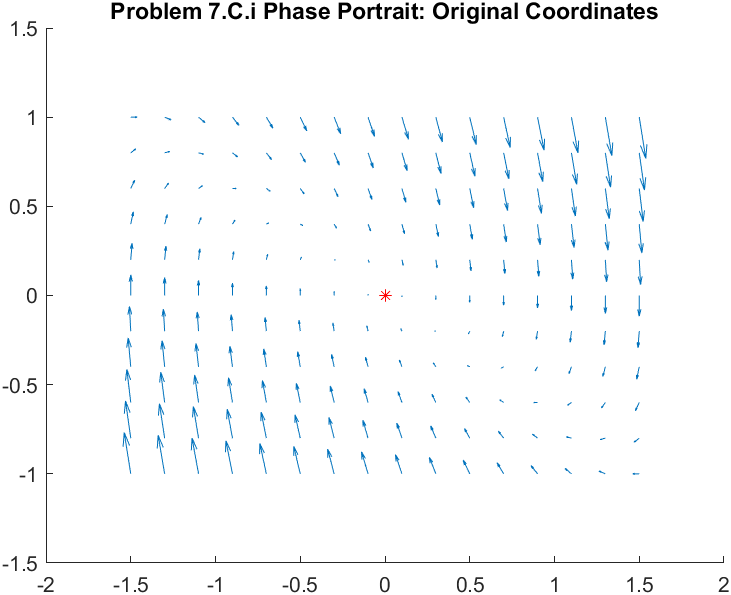
\includegraphics[width=\linewidth]{/prob7_img/7_C_i_Original}
  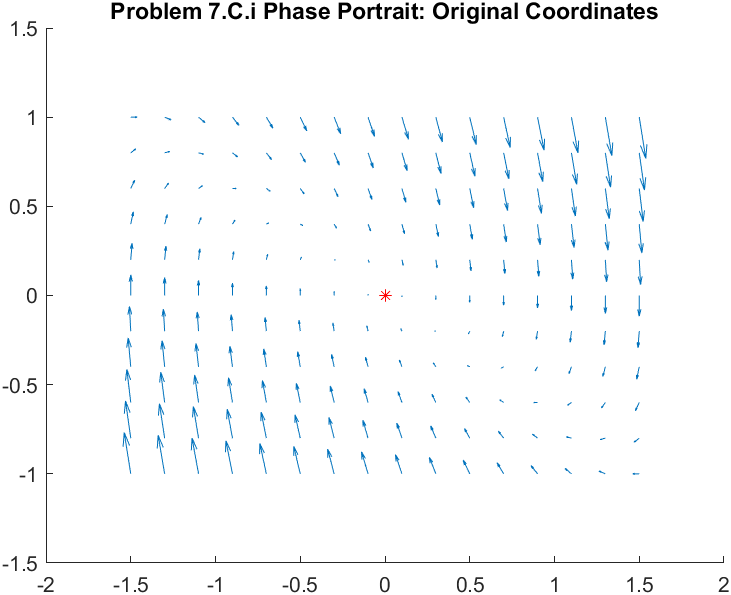
\includegraphics[width=\textwidth,height=.45\textheight,keepaspectratio]{/prob7_img/7_C_i_Original}
\end{figure}

\begin{figure}[h]
  \centering
  % 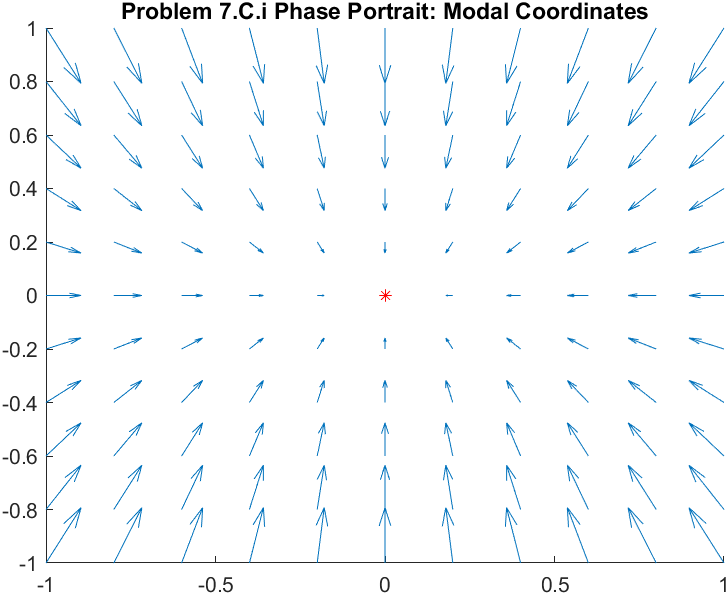
\includegraphics[width=\linewidth]{/prob7_img/7_C_i_modal}
  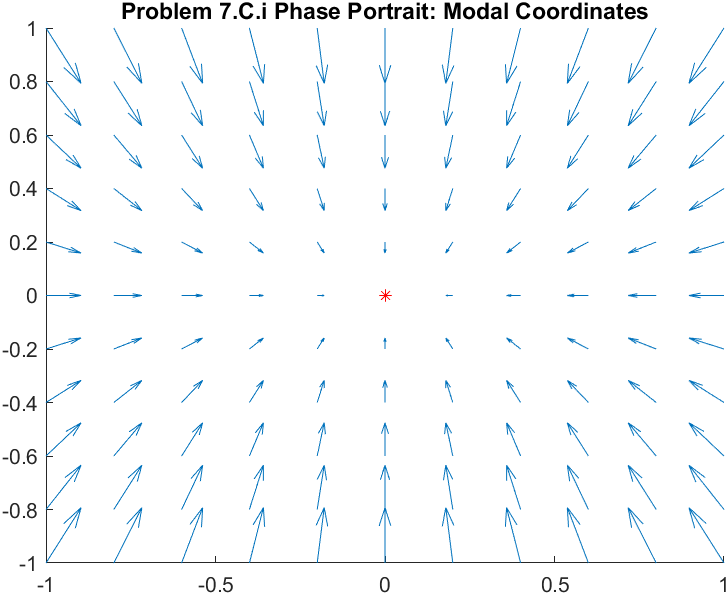
\includegraphics[width=\textwidth,height=.45\textheight,keepaspectratio]{/prob7_img/7_C_i_modal}

\end{figure}

\begin{figure}[h]
  \centering
  % 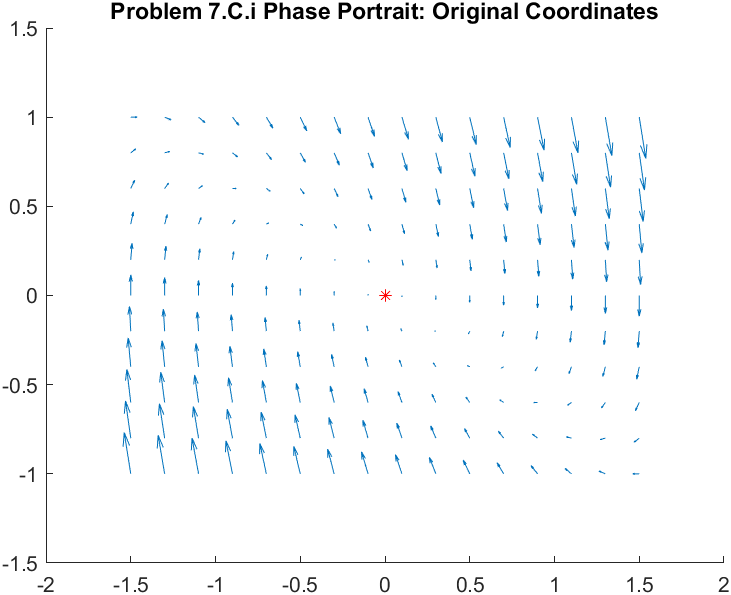
\includegraphics[width=\linewidth]{/prob7_img/7_C_i_Original}
  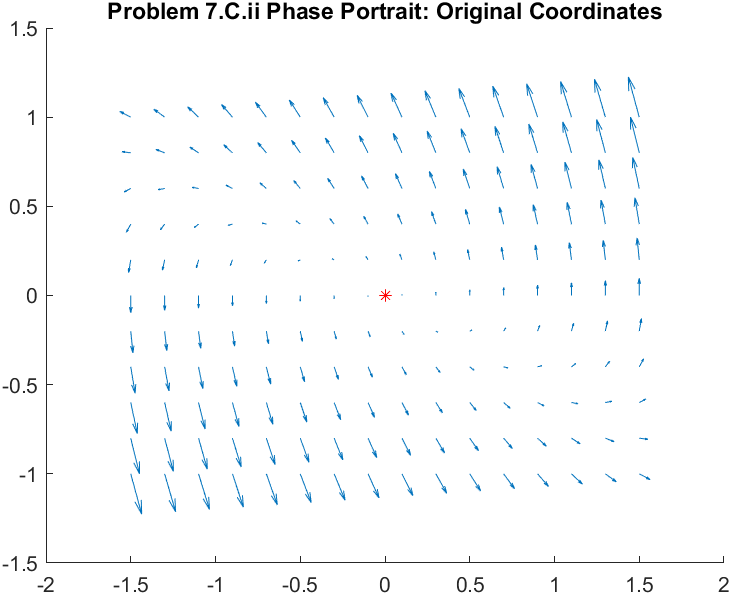
\includegraphics[width=\textwidth,height=.45\textheight,keepaspectratio]{/prob7_img/7_C_ii_Original}
\end{figure}

\begin{figure}[h]
  \centering
  % 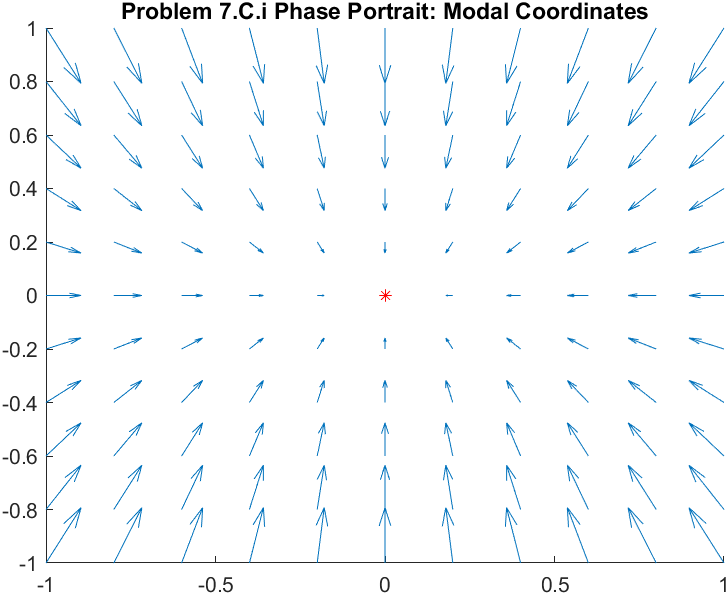
\includegraphics[width=\linewidth]{/prob7_img/7_C_i_modal}
  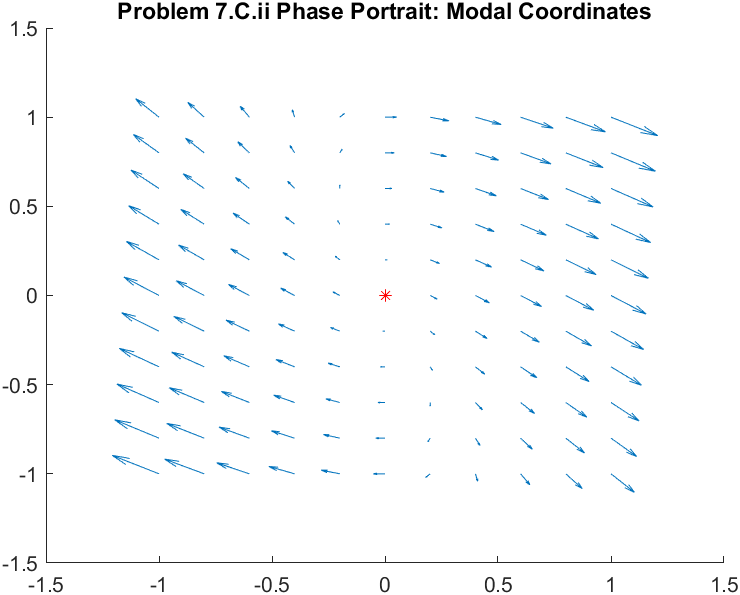
\includegraphics[width=\textwidth,height=.45\textheight,keepaspectratio]{/prob7_img/7_C_ii_modal}

\end{figure}

\begin{figure}[h]
  \centering
  % 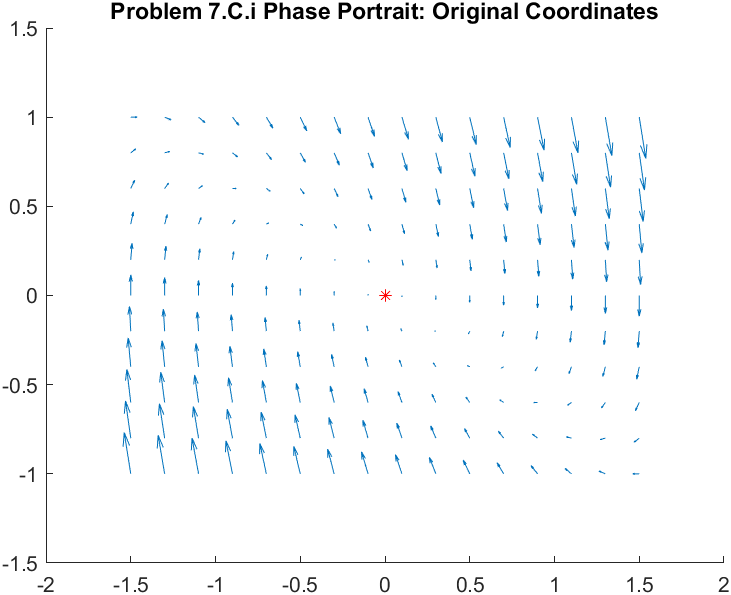
\includegraphics[width=\linewidth]{/prob7_img/7_C_i_Original}
  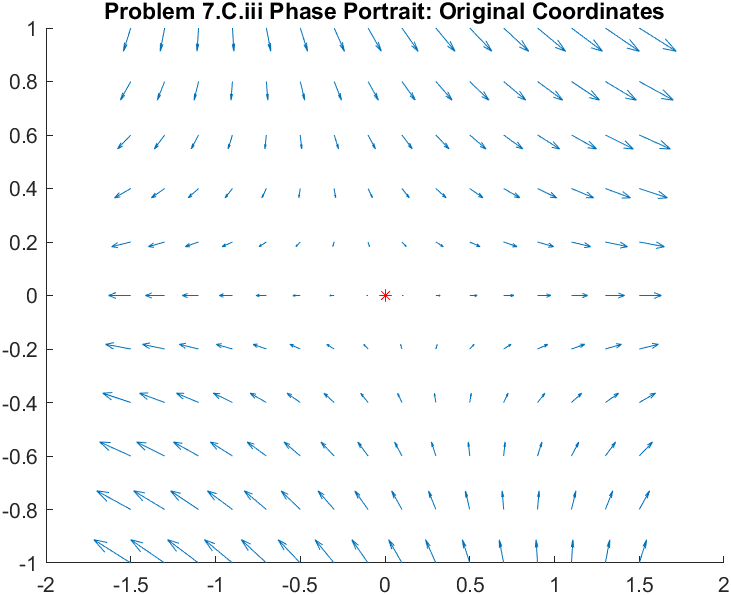
\includegraphics[width=\textwidth,height=.45\textheight,keepaspectratio]{/prob7_img/7_C_iii_Original}
\end{figure}

\begin{figure}[h]
  \centering
  % 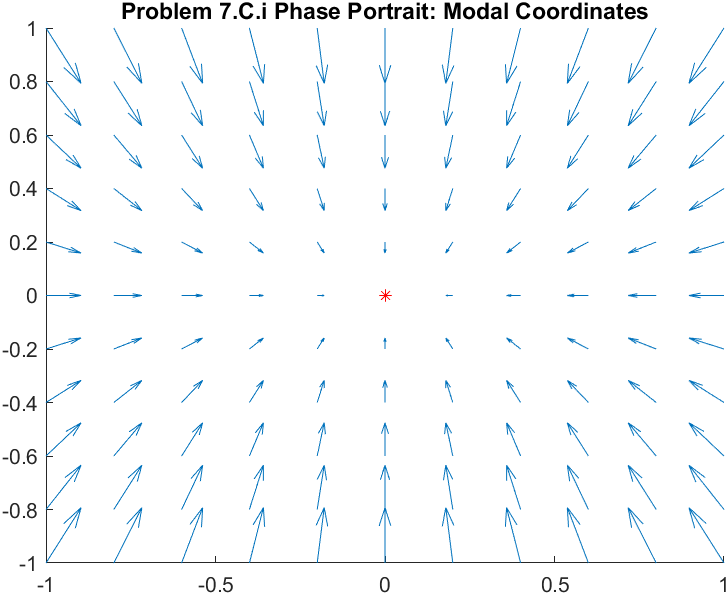
\includegraphics[width=\linewidth]{/prob7_img/7_C_i_modal}
  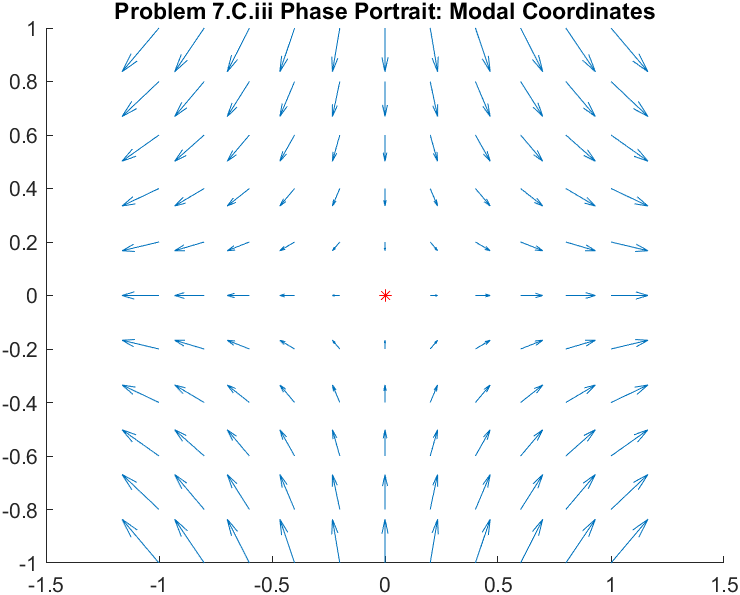
\includegraphics[width=\textwidth,height=.45\textheight,keepaspectratio]{/prob7_img/7_C_iii_modal}

\end{figure}

\begin{figure}[h]
  \centering
  % 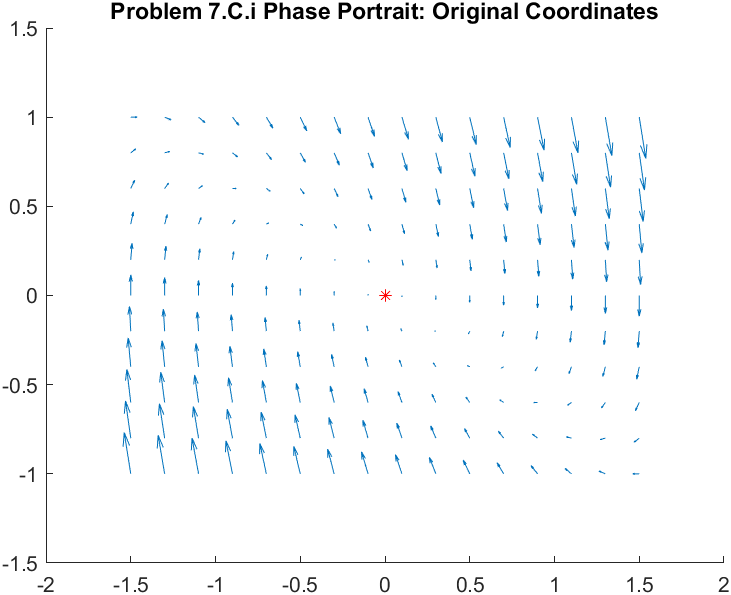
\includegraphics[width=\linewidth]{/prob7_img/7_C_i_Original}
  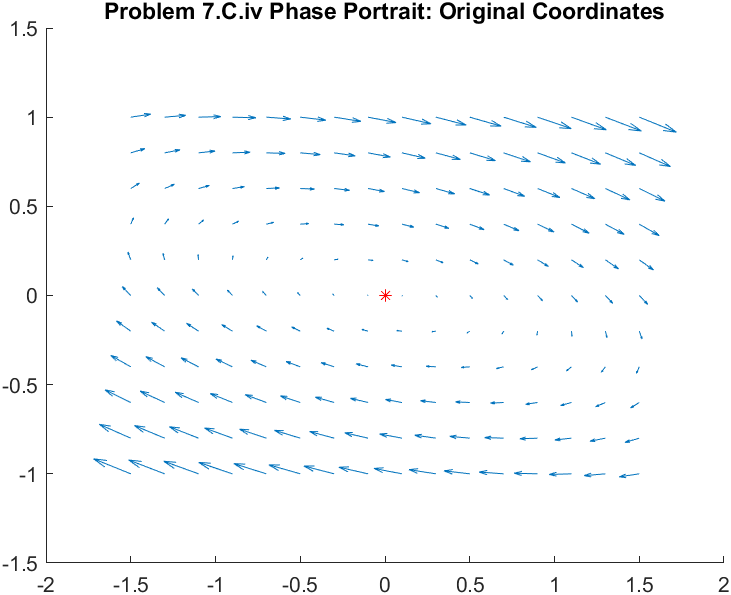
\includegraphics[width=\textwidth,height=.45\textheight,keepaspectratio]{/prob7_img/7_C_iv_Original}
\end{figure}

\begin{figure}[h]
  \centering
  % 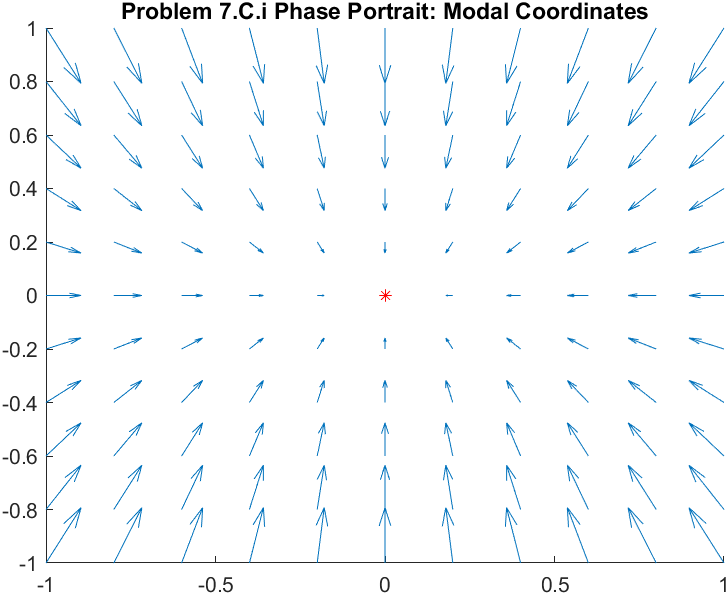
\includegraphics[width=\linewidth]{/prob7_img/7_C_i_modal}
  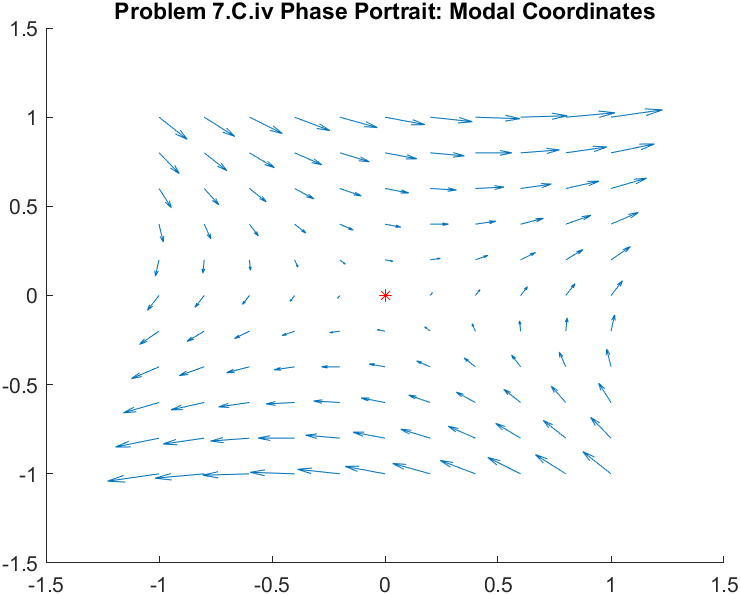
\includegraphics[width=\textwidth,height=.45\textheight,keepaspectratio]{/prob7_img/7_C_iv_modal}

\end{figure}

\begin{figure}[h]
  \centering
  % 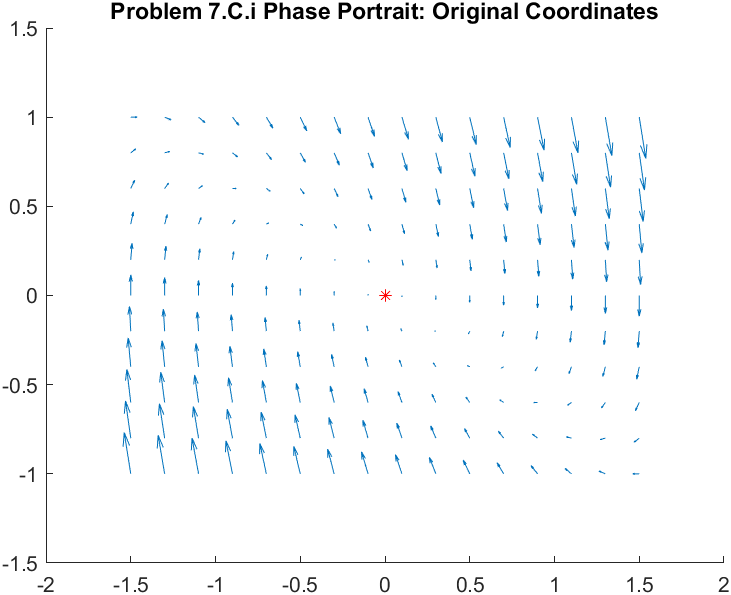
\includegraphics[width=\linewidth]{/prob7_img/7_C_i_Original}
  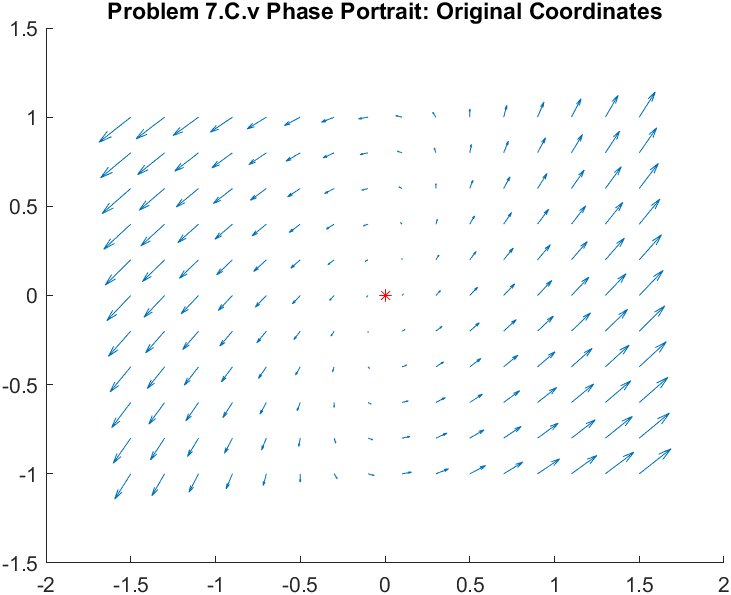
\includegraphics[width=\textwidth,height=.45\textheight,keepaspectratio]{/prob7_img/7_C_v_Original}
\end{figure}

\begin{figure}[h]
  \centering
  % 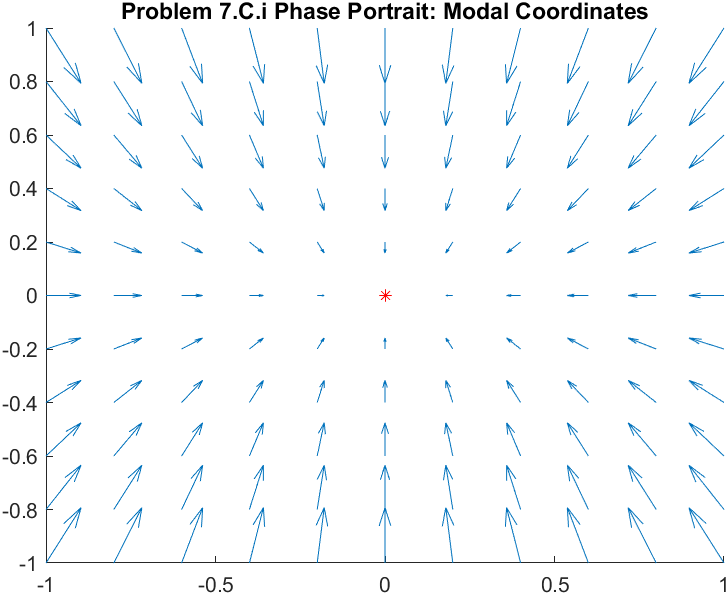
\includegraphics[width=\linewidth]{/prob7_img/7_C_i_modal}
  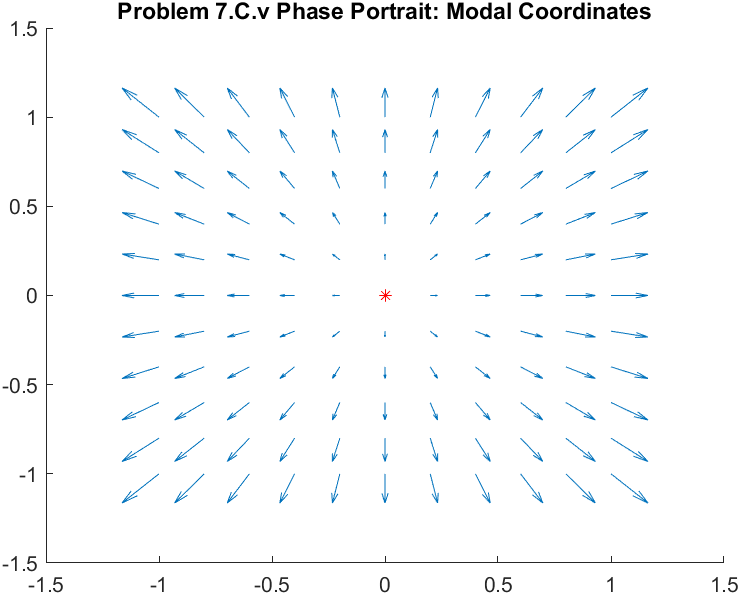
\includegraphics[width=\textwidth,height=.45\textheight,keepaspectratio]{/prob7_img/7_C_v_modal}

\end{figure}
